\documentclass[11pt,a4paper]{article}
\usepackage[margin=25mm,headheight=15pt]{geometry}
\usepackage[T1]{fontenc}
\usepackage{newtxtext}
\usepackage{amsmath,amsthm}
\usepackage{newtxmath}
\usepackage{microtype,mathtools,bm}
\usepackage{xcolor,graphicx,booktabs,array,enumitem}
\usepackage{fancyhdr,xurl}
\usepackage[colorlinks=true,linkcolor=blue!45!black,citecolor=blue!45!black,urlcolor=blue!45!black]{hyperref}
\usepackage{aliascnt}
\usepackage[nameinlink,noabbrev]{cleveref}
\definecolor{ink}{RGB}{24,45,70}
\definecolor{paperblue}{RGB}{238,243,248}
\pagestyle{fancy}\fancyhf{}
\fancyhead[L]{\small\textsc{Complex transseries reversion}}
\fancyhead[R]{\small 4 October 2026}
\fancyfoot[C]{\thepage}
\setlength{\parindent}{1.25em}
\setlength{\parskip}{3pt}
\setlength{\emergencystretch}{2em}
\setcounter{tocdepth}{2}
\numberwithin{equation}{section}
\newtheorem{theorem}{Theorem}[section]
\newaliascnt{lemma}{theorem}
\newtheorem{lemma}[lemma]{Lemma}
\aliascntresetthe{lemma}
\newaliascnt{proposition}{theorem}
\newtheorem{proposition}[proposition]{Proposition}
\aliascntresetthe{proposition}
\newaliascnt{corollary}{theorem}
\newtheorem{corollary}[corollary]{Corollary}
\aliascntresetthe{corollary}
\theoremstyle{definition}
\newaliascnt{definition}{theorem}
\newtheorem{definition}[definition]{Definition}
\aliascntresetthe{definition}
\newaliascnt{example}{theorem}
\newtheorem{example}[example]{Example}
\aliascntresetthe{example}
\theoremstyle{remark}
\newaliascnt{remark}{theorem}
\newtheorem{remark}[remark]{Remark}
\aliascntresetthe{remark}
\newcommand{\C}{\mathbb C}
\newcommand{\R}{\mathbb R}
\newcommand{\N}{\mathbb N}
\newcommand{\e}{\mathrm e}
\newcommand{\ii}{\mathrm i}
\newcommand{\D}{\mathbb D}
\newcommand{\id}{\operatorname{id}}
\newcommand{\ord}{\operatorname{ord}}
\newcommand{\Res}{\operatorname{Res}}
\newcommand{\Log}{\operatorname{Log}}
\newcommand{\rad}{\operatorname{rad}_0}
\newcommand{\scv}{s_{\mathrm c}}
\newcommand{\qcv}{q_{\mathrm c}}
\newcommand{\norm}[1]{\left\lVert#1\right\rVert}
\newcommand{\abs}[1]{\left|#1\right|}
\newcommand{\repo}{\texttt{ProveIt}}
\hypersetup{pdftitle={Complex Transseries Reversion: Exact Radii and Sheet-Selective Critical Geometry},pdfauthor={Research report prepared for Vladimir Reshetnikov},pdfsubject={Sectorial transseries, compositional inversion, Lambert perturbations, coefficient asymptotics}}
\begin{document}
\hypersetup{pageanchor=false}
\begin{titlepage}
\color{ink}
\vspace*{12mm}
{\large\scshape Research in transseries and complex asymptotics\par}
\vspace{12mm}
{\fontsize{29}{34}\selectfont\bfseries Complex Transseries\par Reversion\par}
\vspace{7mm}
{\Large Exact radii, sheet-selective critical geometry,\par and late exponential sectors\par}
\vspace{13mm}
{\large A continuation of the \repo{} transseries program\par}
\vspace{4mm}
{Research report prepared for Vladimir Reshetnikov\par 4 October 2026\par}
\vspace{12mm}
\color{black}
\begin{abstract}
Series reversion on the complex plane requires more information than a formal list of transmonomials: a compatible substitution chart, an analytic realization, and a selected inverse sheet. We develop these layers separately and prove a quantitative result connecting them. If
\[
 Q(s)=-s\exp(s+V(s)),\qquad V(0)=0,
 \qquad \sup_{|s|\leq1+\delta}|V(s)|\leq\frac{\delta^2}{1000},
\]
where $0<\delta\leq\tfrac12$, then the inverse germ $s(0)=0$ has exactly one singularity on its circle of convergence. It is the simple critical value near $\e^{-1}$, and the radius is its modulus, even for complex-valued perturbations without coefficient positivity. The proof uses a circle through the perturbed critical point on which $|Q|$ has a unique minimum.

This determines the exact radius in a sufficiently large-core regime left unresolved in an inspected \repo{} report. It also gives all-order late-sector asymptotics, a boundary truncation law, and a double-scaling law showing how a small curvature correction changes high-order sectors by an order-one factor. A fully explicit entire example has a critical value on another sheet more than $10^{1081}$ times closer to the origin than the selected branch's convergence radius. We extend the normalization to nonlinear exponential actions and analytic prefactors, explain sectorial and Stokes gluing, and provide exact symbolic checks and high-precision diagnostics.
\end{abstract}
\vfill
\noindent\small\textbf{Status.} The main geometric theorem and its consequences are proved here. Classical reversion, resurgence closure, and square-root transfer are credited. No claim of a new universal field of complex transseries, a general summability theorem, independent priority, or Lean verification is made.
\end{titlepage}
\hypersetup{pageanchor=true}
\pagenumbering{roman}
\begingroup
\small
\setlength{\parskip}{0pt}
\tableofcontents
\endgroup
\newpage
\pagenumbering{arabic}

\section{The problem and the specific advance}
\label{sec:intro}
Let a function or formal expansion be given in a variable tending to infinity,
\begin{equation}
 F(z)=F_0(z)+E(z),\qquad w=F(z).
 \label{eq:original}
\end{equation}
The purpose of reversion is to construct a selected solution $z=G(w)$ and to understand which of its expansions are formal, asymptotic, convergent, or summable. In the complex setting there is no useful answer that suppresses the domain and branch data. Even the comparison between $\e^{-z}$ and $1$ changes when a direction is rotated through the imaginary axis. A logarithm requires a sheet, and a locally invertible map may have many globally different inverse branches.

The most useful continuation of the existing program is therefore not another unrestricted closure assertion. It is a theorem that identifies the precise analytic obstruction for a broad and checkable family of inverse transseries, together with a framework explaining where that theorem applies.

\subsection{Repository audit and the unresolved radius question}
The inspected repository contains a consolidated polynomial--logarithmic calculus, exact-core reversion formulas, support-control arguments, analytic residual estimates, nonlinear Stokes transport, and moving-fold analysis. The canonical consolidated source is in
\begin{quote}\small\path{Analysis/Transseries/docs/series-and-transseries/Transseries_And_Inversion/}.
\end{quote}
The report \emph{Nonlinear Stokes Transport under Logarithmic Inversion} studies, in its normalized coordinates,
\begin{equation}
 \psi_g(s)+q\e^{-s}=0,
 \qquad Q_g(s)=-\e^s\psi_g(s),
 \label{eq:repo-normalization}
\end{equation}
with $\psi_g(s)=s+O(g^{-2})$ on a fixed complex disk larger than the unit disk. Its theorem labelled \texttt{thm:radius} proves
\begin{equation}
 (1-\vartheta_g)\e^{-1}\leq R_g\leq q_{\mathrm c}(g),
 \qquad R_g=\e^{-1}+O(g^{-2}),
 \label{eq:old-radius}
\end{equation}
but deliberately does not identify the real fold with the exact nearest singularity of the selected Taylor branch at every sufficiently large finite $g$ \cite{repo-stokes}. The README repeats this limitation. Nearby inspected material also distinguishes asymptotic radius information from a sheet-specific exact radius \cite{repo-moments}.

\Cref{thm:lambert} supplies the missing analytic argument. Under the stated complex-uniform hypotheses, it implies
\begin{equation}
 \boxed{R_g=q_{\mathrm c}(g)\quad\text{for every sufficiently large real }g.}
 \label{eq:resolution}
\end{equation}
The qualification ``sufficiently large'' is essential. The theorem does not establish the claim for all smaller $g$, nor does it replace global inverse-branch classification.

The repository paths and searches used for this comparison were inspected on 4 October 2026; the pinned comparison revision returned by code search is
\begin{quote}\small\texttt{6cb1d86f19ebf9f54c8d985b141b84233b6eab66}.
\end{quote}
This is a targeted audit, not a line-by-line verification of the entire repository or a complete priority search.

\subsection{What is proved and what is inherited}
The new mathematical package developed here consists of the critical-circle theorem, its exact-radius consequence for the logarithmic-core question, the sheet-selective counterexample, and the resulting uniform late-sector and boundary-layer conclusions. The explicit constant $1/1000$ is conservative; its purpose is to make the hypothesis verifiable, not optimal.

Several ingredients are classical. Lagrange--B\"urmann reversion already supplies coefficients. Sauzin proves resurgent and summable nonlinear closure in precise classes, including functional inversion \cite{sauzin}. The Lambert $W$ function already supplies the unperturbed square-root model \cite{dlmf}. Singularity analysis already transfers a proved dominant local expansion to coefficient asymptotics \cite{fs}. Our task is to establish the missing dominance and sheet-selection hypotheses, and then exploit them. Independent novelty of every consequence is not asserted.

\section{What a complex transseries inversion datum contains}
\label{sec:framework}
\subsection{Three distinct mathematical objects}
A formal transseries with complex coefficients is not automatically an analytic function. A sectorial asymptotic expansion is not automatically a uniquely determined function. A convergent expansion in an exponential marker does not imply convergence of the inverse-power expansions within its coefficients.

For example, one may have
\begin{equation}
 G(w,\sigma)=G_0(w)+\sum_{n\geq1}\sigma^n\e^{-n\Phi(G_0(w))}C_n(w),
 \label{eq:two-layers}
\end{equation}
where the sum over $n$ converges locally in $\sigma$, but the expansions of $C_n(w)$ in powers of $w^{-1}$ diverge. Throughout this report, ``radius'' means the Taylor radius in the stated amplitude variable, unless another variable is explicitly named.

\begin{definition}[Sectorial inversion datum]
A sectorial inversion datum consists of a sector or logarithmic covering chart $S$, a specified branch of each logarithm and power, a formal differential algebra with admissible substitutions, an analytic realization $F$ on $S$, and a selected local inverse germ. A summation operator, when used, is additional structure with explicitly stated closure and compatibility properties.
\end{definition}

For a sector $S(R;\theta_-,\theta_+)$, powers mean $z^\beta=\exp(\beta\Log z)$ with the chosen logarithm. If the angular width or continuation requires it, $S$ is a subset of the logarithmic covering surface rather than a subset of the punctured plane.

Merely adjoining complex constants to a real transseries field does not by itself solve oscillatory composition problems. Direction-dependent compatibility of composition is already an explicit issue in the complex-transseries literature \cite{vdh-complex}. We make it part of the data instead of assuming it away.

\subsection{Action cones and local finiteness}
Suppose a finite set of actions $A_1,\ldots,A_m\in\C$ satisfies
\begin{equation}
 \inf_{\theta\in I}\Re(A_j\e^{\ii\theta})\geq c>0
 \quad(1\leq j\leq m)
 \label{eq:cone}
\end{equation}
on a closed angular interval $I$. Products of the markers $\e^{-A_jz}$ have actions $\sum_j\alpha_jA_j$. A bound on the projected action gives a bound on $|\alpha|$, hence only finitely many multiindices occur below each action budget. Coincident actions may be collected into finite blocks. This is a sufficient support mechanism for the outer exponential expansion; coefficient-algebra support conditions remain separate.

For countably many actions, a uniform positive lower bound alone does not give finite action budgets: infinitely many generators can already lie below one budget. Requiring only finitely many generators below each budget does. Alternatively, a weighted analytic completion may converge even when the formal support mechanism fails. These two alternatives must not be conflated. In particular, a weighted analytic inversion result is not automatically a countable-action resurgence theorem.

\subsection{Two obstructions to an unrestricted statement}
The transmonomial $\e^{-z^2}$ decays on some sectors and grows on others, so one small-perturbation chart cannot describe all directions at once. More sharply, real-axis smallness is not enough even for local inversion. On the positive real axis,
\begin{equation}
 F(x)=x+\e^{-x}\sin(\e^{2x})=x+o(1),
\end{equation}
but
\[
 F'(x)=1-\e^{-x}\sin(\e^{2x})+2\e^x\cos(\e^{2x})
\]
has infinitely many zeros. Indeed it has opposite signs at the interlacing points where $\e^{2x}$ is an even or odd multiple of $\pi$, once $x$ is large. Thus a real-axis error estimate does not supply a uniform inverse chart. Complex-uniform analyticity and derivative control are substantive hypotheses.

\section{A formal reversion theorem with an explicit derivative budget}
\label{sec:formal}
This section records a sufficient formal framework. It is not a characterization of every well-based or oscillatory transseries field.

Let $\mathcal A$ be a commutative differential $\C$-algebra with a separated complete decreasing filtration $\mathcal F_r$, $r\in\R$, such that
\begin{equation}
 \mathcal F_r\mathcal F_t\subseteq\mathcal F_{r+t},
 \qquad D\mathcal F_r\subseteq\mathcal F_{r-\kappa}
 \label{eq:filtration}
\end{equation}
for some $\kappa\geq0$. Completeness is with respect to $r\to+\infty$. We work in a substitution chart with a distinguished variable and associative Taylor substitution. Write
\[
 T_h(f)=\sum_{k\geq0}\frac{D^kf}{k!}h^k.
\]
The estimates below ensure the required sums converge in the filtration. Associativity is the usual universal Taylor-substitution identity in such a chart, not a blanket assertion about undefined compositions.

\begin{theorem}[Filtered near-identity reversion]
\label{thm:filtered}
If $f\in\mathcal F_\lambda$ and $\lambda>\kappa$, there is a unique $h\in\mathcal F_\lambda$ satisfying $h=-T_h(f)$. It is the near-identity inverse displacement for $\id+f$, and
\begin{equation}
 h=\sum_{n\geq1}\frac{(-1)^n}{n!}D^{n-1}(f^n).
 \label{eq:lagrange-differential}
\end{equation}
The $n$th summand belongs to $\mathcal F_{\lambda+(n-1)(\lambda-\kappa)}$. Picard iteration starting at zero gains at least $\lambda-\kappa$ in filtration order at every step.
\end{theorem}
\begin{proof}
For $h\in\mathcal F_\lambda$, the $k$th Taylor term is in
$\mathcal F_{\lambda+k(\lambda-\kappa)}$, so $T_h(f)$ is defined and lies in $\mathcal F_\lambda$. If $h-\widetilde h\in\mathcal F_r$, then
\[
 h^k-\widetilde h^k=(h-\widetilde h)
 \sum_{j=0}^{k-1}h^j\widetilde h^{k-1-j}
\]
shows that the $k\geq1$ difference term belongs to
$\mathcal F_{r+k(\lambda-\kappa)}$. Hence the fixed-point map improves differences by $\lambda-\kappa$. Its iterates are Cauchy; completeness gives a fixed point, and separatedness gives uniqueness.

Introduce an auxiliary formal parameter $t$ in $h_t=-tT_{h_t}(f)$. The formal Lagrange identity gives
$[t^n]h_t=(-1)^nD^{n-1}(f^n)/n!$. This identity is universal in the differential polynomials in $f,Df,\ldots$; it follows either by formal residues or the ordinary Lagrange identity with Taylor coefficients treated as indeterminates. The bound in \eqref{eq:filtration} is
$n\lambda-(n-1)\kappa$, so evaluation at $t=1$ is legitimate. This proves \eqref{eq:lagrange-differential}.

The fixed-point equation gives $(\id+f)\circ(\id+h)=\id$. Applying the same construction to $h$ gives a right inverse of $\id+h$. Associativity then makes the already obtained right inverse two-sided.
\end{proof}

The condition $\lambda>\kappa$ is sufficient, not necessary. In exponential-action filtrations, differentiation often has zero action cost; in finer coefficient filtrations it can have a nonzero cost. Non-Archimedean Hahn supports may be summable for reasons not captured by a real-indexed complete filtration, and require a separate summability proof.

\subsection{Exact-core reversion}
Suppose $F_0$ has a chosen inverse $G_0$. Set
\[
 H(w)=E(G_0(w)),\qquad t=F_0(z).
\]
Then $w=t+H(t)$ and $G=G_0\circ(\id+H)^{-1}$. Under the corresponding admissibility hypotheses, Lagrange--B\"urmann gives
\begin{equation}
 G(w)=G_0(w)+\sum_{n\geq1}\frac{(-1)^n}{n!}
 D_w^{n-1}\!\left(G_0'(w)H(w)^n\right).
 \label{eq:core-lagrange}
\end{equation}
This reorganizes scale-changing inversion into a known core followed by a near-identity problem. It is a classical tool already central to the repository, not a newly claimed formula.

For $E=\sum_{j=1}^m\sigma_jE_j$, the coefficient of $\bm\sigma^\alpha$, with $|\alpha|=n\geq1$, is
\begin{equation}
 \frac{(-1)^n}{\alpha!}D_w^{n-1}
 \left(G_0'(w)\prod_{j=1}^m(E_j\circ G_0)^{\alpha_j}\right).
 \label{eq:mixed}
\end{equation}
In particular, actions are transported as $\Phi_j\circ G_0$ before any further expansion. Replacing this exact transported action by an insufficient truncation can change the exponential scale.

\section{Analytic realization and residual certification}
\label{sec:certificates}
Formal reversion supplies a candidate. A short analytic argument can certify a selected local root without presupposing convergence of all the coefficient expansions.

\begin{proposition}[Derivative-disk certificate]
\label{prop:certificate}
Let $F$ be holomorphic on a neighborhood of $\overline{D(z_0,\rho)}$, let $c=F'(z_0)\neq0$, and suppose
\[
 \sup_{|z-z_0|\leq\rho}|F'(z)-c|\leq\eta|c|,
 \quad 0\leq\eta<1,
 \quad |F(z_0)-w|<(1-\eta)|c|\rho.
\]
Then $F(z)=w$ has exactly one root in $D(z_0,\rho)$, and
\begin{equation}
 |z-z_0|\leq\frac{|F(z_0)-w|}{(1-\eta)|c|}.
 \label{eq:certificate}
\end{equation}
\end{proposition}
\begin{proof}
On the disk, integration along a segment gives
$|F(z_0+h)-F(z_0)-ch|\leq\eta|c||h|$. On the boundary, compare $F(z_0+h)-w$ with $ch$: the sum of the constant residual and the nonlinear remainder is strictly smaller than $|c|\rho$. Rouch\'e's theorem gives one zero, counted with multiplicity. The same segment estimate at the root gives \eqref{eq:certificate}.
\end{proof}

The estimate degenerates near a fold because the relevant derivative tends to zero. The correct local variable there is a square root, not a better-conditioned version of the same linear inverse estimate. The main theorem will identify that fold and show when it is the actual dominant obstruction.

If a specified summation map commutes with the admitted algebraic operations, derivatives, and substitutions, and the analytic inverse is uniquely selected by such a disk, the summed formal inverse agrees with that analytic inverse. This is a compatibility statement conditional on the summation hypotheses. In the closed-discrete resurgent setting, the necessary nonlinear closure results are established in \cite{sauzin}; no extension to all transseries is inferred merely from formal solvability.

\section{The critical-circle theorem}
\label{sec:main}
\begin{theorem}[Lambert-stable, sheet-selective exact radius]
\label{thm:lambert}
Let $0<\delta\leq\tfrac12$, let $V$ be holomorphic on a neighborhood of $\overline{D(0,1+\delta)}$, and assume
\begin{equation}
 V(0)=0,\qquad
 \norm{V}_{1+\delta}:=\sup_{|s|\leq1+\delta}|V(s)|
 \leq\epsilon,\qquad \epsilon\leq\delta^2/1000.
 \label{eq:smallV}
\end{equation}
Define
\begin{equation}
 Q(s)=-s\exp(s+V(s)),\qquad
 H(s)=1+s+sV'(s).
 \label{eq:QH}
\end{equation}
There is exactly one critical point $\scv$ in $|s+1|<\delta/4$, and it is simple. Put $\qcv=Q(\scv)$ and $\tau=|\scv|$. Then:
\begin{enumerate}[label=(\roman*),leftmargin=2em]
\item On $|s|=\tau$, $|Q(s)|\geq|\qcv|$, with equality only at $s=\scv$.
\item The inverse germ $s(q)$ satisfying $s(0)=0$ is holomorphic for $|q|<|\qcv|$ and obeys $|s(q)|<\tau$.
\item Its Taylor radius is exactly $|\qcv|$. The only singularity of this germ on that circle is $\qcv$, and it is a square-root branch point.
\item The germ extends through every other point of the circle and to a slit neighborhood of $\qcv$. In the variable $q/\qcv$ it has a $\Delta$-domain extending beyond the unit circle.
\end{enumerate}
If $V$ is real on the real axis, $\scv<0$, $\qcv>0$, and the radius is $\qcv$ itself. No positivity of the Taylor coefficients of $V$ or of the inverse is assumed.
\end{theorem}

\subsection{Locating the critical point}
\begin{proof}[Proof of \cref{thm:lambert}, critical-point part]
On $|s|\leq1+\delta/4$, Cauchy's estimates with radius $\delta/2$ give
\begin{equation}
 |V'(s)|\leq\frac{2\epsilon}{\delta},\qquad
 |V''(s)|\leq\frac{8\epsilon}{\delta^2}.
 \label{eq:cauchyV}
\end{equation}
On $|s+1|=\delta/4$, $|s|\leq9/8$, and
\[
 |sV'(s)|\leq\frac{9\epsilon}{4\delta}<\frac\delta4.
\]
Rouch\'e applied to $H(s)=(1+s)+sV'(s)$ gives exactly one zero in this circle, counted with multiplicity. It is consequently simple. Since
$Q'(s)=-\exp(s+V(s))H(s)$, this is a simple critical point of $Q$. In particular,
\begin{equation}
 |\scv+1|\leq\frac{9\epsilon}{4\delta},\qquad
 \frac78<\tau<\frac98.
 \label{eq:sc-bound}
\end{equation}
Also
\begin{equation}
 H'(\scv)=1+V'(\scv)+\scv V''(\scv),
 \qquad |H'(\scv)-1|\leq10\epsilon/\delta^2\leq0.01.
 \label{eq:Hprime}
\end{equation}
\end{proof}

\subsection{The angular minimum, including complex perturbations}
\begin{proof}[Proof of part (i)]
On $s=\tau\e^{\ii\theta}$, write
\begin{equation}
 \log|Q(s)|=\log\tau+h(\theta),\qquad
 h(\theta)=\tau\cos\theta+\Re V(\tau\e^{\ii\theta}).
 \label{eq:angular}
\end{equation}
For $|\theta-\pi|\leq\pi/3$, interpreted modulo $2\pi$,
\[
 h''(\theta)=-\tau\cos\theta+
 \Re\{-sV'(s)-s^2V''(s)\}.
\]
The absolute value of the perturbation is at most
\[
 \frac{9\epsilon}{4\delta}+\frac{81\epsilon}{8\delta^2}
 \leq\frac{12\epsilon}{\delta^2}\leq0.012.
\]
Hence $h''\geq7/16-0.012>0$ on this interval. Outside the interval,
\[
 h(\theta)-h(\pi)\geq\frac\tau2-2\epsilon>0.
\]
Thus the global minimum lies in the interval of strict convexity and is unique there.

Let $\theta_{\mathrm c}=\arg\scv$ near $\pi$. The bound \eqref{eq:sc-bound} puts it inside that interval. The critical equation gives $\scv(1+V'(\scv))=-1$, and therefore
\[
 h'(\theta_{\mathrm c})=
 \Re\{\ii\scv(1+V'(\scv))\}=0.
\]
The unique minimum is precisely $s=\scv$. This proves part (i). The argument uses the critical equation rather than conjugation symmetry, which is why it also works for genuinely complex perturbations.
\end{proof}

\begin{figure}[htbp]
\centering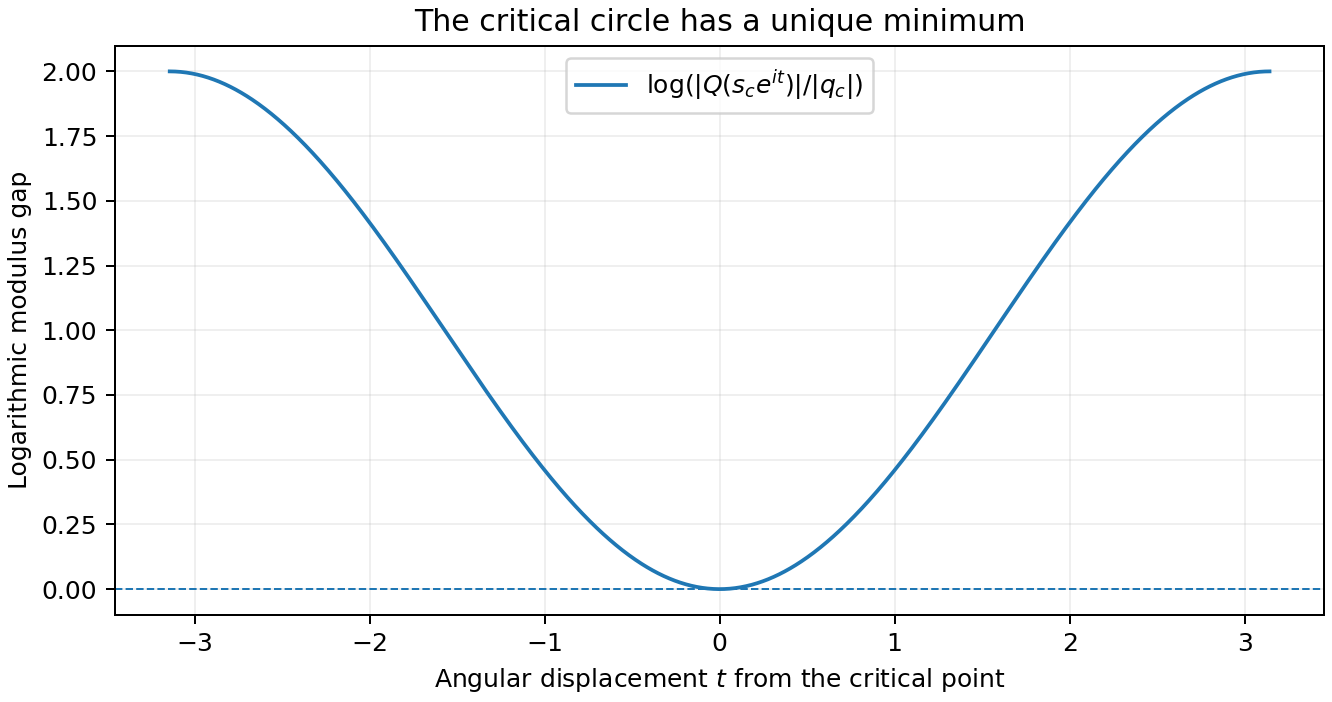
\includegraphics[width=0.91\linewidth]{figures/critical_circle.png}
\caption{A diagnostic for $V(s)=(5+5\ii)10^{-5}s^2$. The plotted logarithmic modulus gap is nonnegative and vanishes at the critical point. The theorem proves this inequality on the whole circle; sampling is only an illustration.}
\label{fig:circle}
\end{figure}

\subsection{Selecting the inverse sheet}
\begin{proof}[Proof of parts (ii)--(iv)]
For $|q|<|\qcv|$, part (i) permits Rouch\'e's theorem on $|s|=\tau$ for $Q(s)-q$ and $Q(s)$. The latter has exactly one zero in the disk, a simple zero at $0$. Thus $Q(s)-q$ has one zero counted with multiplicity. It is simple, varies holomorphically with $q$, and agrees with the inverse germ at $0$. Uniqueness patches the local solutions across the whole amplitude disk.

It remains important to show that the critical point actually lies on the boundary of \emph{this} sheet. Put
\begin{equation}
 A_2=-\frac{Q''(\scv)}{2\qcv}
     =-\frac{H'(\scv)}{2\scv}.
 \label{eq:A2}
\end{equation}
By \eqref{eq:sc-bound}--\eqref{eq:Hprime}, $A_2$ is close to $1/2$. There is a square root
\begin{equation}
 b_1=A_2^{-1/2}=\sqrt{-\frac{2\scv}{H'(\scv)}}
 \label{eq:b1}
\end{equation}
close to $\sqrt2$. In particular $\Re(b_1\overline{\scv})<0$. To see that the bounds suffice quantitatively, $|\scv+1|\leq0.001125$ and $|H'-1|\leq0.01$ imply
$|(-\scv/H')-1|<0.012$; the square root near $1$ then differs from $1$ by less than $0.012$. This leaves the displayed real part strictly negative.

The analytic factorization at a simple critical point gives two local roots at $q=(1-t)\qcv$, $t>0$ small:
\begin{equation}
 s=\scv\pm b_1\sqrt t+O(t).
 \label{eq:local-root-pair}
\end{equation}
The plus root lies inside $|s|<\tau$ and the minus root outside, because the first variation of $|s|^2$ is $\pm2\Re(b_1\overline{\scv})\sqrt t$. The plus root must therefore be the already selected inverse. It tends to $\scv$ and cannot extend holomorphically at $\qcv$: differentiating $Q(s(q))=q$ there would give $0=1$. Hence the radius is at most $|\qcv|$, and part (ii) gives equality.

At a boundary point $q_0\neq\qcv$, part (i) says that $Q(s)-q_0$ has no zero on $|s|=\tau$. Its zero count is unchanged from an inward radial perturbation and equals one. The root is simple and the implicit-function theorem continues the selected inverse through $q_0$.

Finally, factor $1-Q(s)/\qcv=(s-\scv)^2A(s)$ with $A(\scv)=A_2\neq0$. The coordinate $u=(s-\scv)\sqrt{A(s)}$ has nonzero derivative and reduces the equation exactly to $u^2=1-q/\qcv$. This gives the local slit continuation. Compactness of the rest of the amplitude circle supplies a finite collection of ordinary continuation neighborhoods. After shrinking their widths, they and the local slit chart form a $\Delta$-domain. Concretely, for some $\eta>0$ and $0<\varphi<\pi/2$, the function of $z=q/\qcv$ extends to
\[
 |z|<1+\eta,\qquad |\arg(z-1)|>\varphi.
\]
The real-valued conclusion follows by conjugation symmetry and the uniqueness of the critical point near $-1$.
\end{proof}

\begin{remark}[What the theorem does not say]
The disk $|s|<\tau$ selects one inverse sheet. It need not contain all preimages of a point under a globally extended $Q$. The entire function $Q$ can have other critical values of much smaller modulus; they need not be singularities of the selected germ. \Cref{sec:foreign} gives an explicit example.
\end{remark}

\section{Late sectors and truncation at the convergence boundary}
\label{sec:late}
Once the dominant singularity has been proved to belong to the selected sheet, classical singularity analysis becomes applicable. Without that geometric step, a formal square-root expansion at a critical point would not suffice.

\subsection{The complete local expansion}
Put
\begin{equation}
 A_j=-\frac{Q^{(j)}(\scv)}{j!\qcv}\quad(j\geq2),
 \qquad t=1-q/\qcv.
 \label{eq:Aj}
\end{equation}
The branch selected in \cref{thm:lambert} has a convergent Puiseux expansion
\begin{equation}
 s(q)=\scv+\sum_{k\geq1}b_k t^{k/2},
 \qquad b_1\text{ near }\sqrt2.
 \label{eq:puiseux}
\end{equation}
The square root of $t$ is positive on the inward real radius $q=(1-t)\qcv$, $t>0$, and is continued from there. The coefficients are
\begin{equation}
 b_k=\frac1k[x^{k-1}]
       \left(A_2+A_3x+A_4x^2+\cdots\right)^{-k/2}.
 \label{eq:bk}
\end{equation}
In particular,
\begin{equation}
 b_1=A_2^{-1/2},\qquad
 b_2=-\frac{A_3}{2A_2^2},\qquad
 b_3=\frac{5A_3^2-4A_2A_4}{8A_2^{7/2}}.
 \label{eq:b123}
\end{equation}
Indeed $t=x^2(A_2+A_3x+\cdots)$ for $x=s-\scv$. Inverting $\sqrt t=x\sqrt{A_2+A_3x+\cdots}$ gives \eqref{eq:bk} by ordinary Lagrange inversion. The chosen square root is the one already fixed by sheet selection, so there is no remaining sign ambiguity.

\begin{theorem}[All-order late-sector asymptotics]
\label{thm:late}
Under \cref{thm:lambert}, write $s(q)=\sum_{n\geq1}c_nq^n$. Then
\begin{align}
 c_n=\qcv^{-n}\bigg[&-\frac{b_1}{2\sqrt\pi}\,n^{-3/2}
 +\left(-\frac{3b_1}{16\sqrt\pi}
           +\frac{3b_3}{4\sqrt\pi}\right)n^{-5/2}
 +O(n^{-7/2})\bigg].
 \label{eq:cn-two}
\end{align}
More generally, for every fixed $M\geq1$ there are computable constants $d_1,\ldots,d_{M-1}$ such that
\begin{equation}
 c_n=-\frac{b_1}{2\sqrt\pi}\qcv^{-n}n^{-3/2}
 \left(1+\frac{d_1}{n}+\cdots+
       \frac{d_{M-1}}{n^{M-1}}+O(n^{-M})\right),
 \label{eq:cn-all}
\end{equation}
where
\begin{equation}
 d_1=\frac38-\frac{3b_3}{2b_1}.
 \label{eq:d1}
\end{equation}
Only finitely many derivatives of $Q$ at $\scv$ are needed for any fixed $d_j$.
\end{theorem}
\begin{proof}
The main theorem gives a $\Delta$-domain, a unique singularity on the convergence circle, and the convergent local expansion \eqref{eq:puiseux}. Apply the transfer theorem for algebraic singularities \cite[Chapter VI]{fs}. The elementary coefficient identity underlying that theorem is
\begin{equation}
 [z^n](1-z)^\beta=
 \frac{\Gamma(n-\beta)}{\Gamma(-\beta)\Gamma(n+1)},
 \qquad \beta\notin\{0,1,2,\ldots\}.
 \label{eq:transfer-gamma}
\end{equation}
For $\beta=1/2$, the gamma ratio is
$n^{-3/2}(1+3/(8n)+O(n^{-2}))$ and $\Gamma(-1/2)=-2\sqrt\pi$. For $\beta=3/2$, the leading term is $n^{-5/2}$ and $\Gamma(-3/2)=4\sqrt\pi/3$. These give \eqref{eq:cn-two}. Integer powers in a finite local expansion are polynomials and have no sufficiently late coefficients. Taking more terms in the local expansion and the gamma ratios proves \eqref{eq:cn-all}. Formula \eqref{eq:bk} gives the finite-jet dependence.
\end{proof}

For the unperturbed map $Q(s)=-s\e^s$, one has $s(q)=W_0(-q)$,
\[
 c_n(0)=-\frac{n^{n-1}}{n!},\quad
 b_1=\sqrt2,\quad b_2=-\frac23,\quad
 b_3=\frac{11\sqrt2}{36}.
\]
Consequently $d_1=-1/12$, in agreement with Stirling's formula. This is a useful sign and normalization check, not a new Lambert identity \cite{dlmf}.

\subsection{Uniformity in analytic families}
\begin{lemma}[Uniform geometry and transfer]
\label{lem:uniform}
Let $V(s,u)$ be jointly holomorphic for $s$ in a neighborhood of $\overline{D(0,1+\delta)}$ and $u$ in a neighborhood of a compact parameter set $K$. Suppose $V(0,u)=0$ and the bound in \eqref{eq:smallV} holds uniformly. Locally in the parameter, $\scv(u)$, $\qcv(u)$, and all $b_k(u)$ are holomorphic. The $\Delta$-domain in $z=q/\qcv(u)$ and the remainder constants in every fixed-order expansion \eqref{eq:cn-all} can be chosen uniformly for $u\in K$.
\end{lemma}
\begin{proof}
The zero of $H$ stays in a fixed small disk about $-1$, and $|H'(\scv)|\geq0.99$. The holomorphic implicit-function theorem supplies $\scv(u)$; substitution gives $\qcv(u)$, which stays away from zero. The square root near $\sqrt2$ fixes a consistent holomorphic choice of $b_1$, and \eqref{eq:bk} gives all further coefficients.

Here are the uniform continuation details. On a fixed neighborhood of the compact set of critical points, joint holomorphy bounds all derivatives needed for the local factorization, while $|A_2|$ is uniformly bounded below. The coordinate used to obtain \eqref{eq:puiseux} therefore has an inverse on a parameter-independent small disk. Away from that local chart, the angular minimum in the proof of \cref{thm:lambert} is uniformly strict on closed angular subsets. On the remaining compact subset of the normalized amplitude circle, the unique root is simple and stays strictly inside its source circle. Compactness and the implicit-function theorem give uniformly wide continuation neighborhoods. They agree with the interior root on their overlaps; shrinking them if necessary gives a single-valued continuation on a common $\Delta$-domain. The local expansions and their remainders are uniformly bounded there. The usual transfer contour can now be chosen independently of $u$, proving the last assertion.
\end{proof}

The lemma concerns an analytic family on a compact parameter range. It does not assert that arbitrary formal dependence on a parameter gives analytic or uniform dependence.

\subsection{Interior and boundary truncation}
Let $S_N(q)=\sum_{n=1}^N c_nq^n$. The root bound $|s(q)|<\tau$ implies, by Cauchy's estimates and a limiting radius,
\begin{equation}
 |c_n|\leq\tau|\qcv|^{-n}.
\end{equation}
For $r=|q/\qcv|<1$ it follows that
\begin{equation}
 |s(q)-S_N(q)|\leq\frac{\tau r^{N+1}}{1-r}.
 \label{eq:rough-tail}
\end{equation}
The late-sector theorem also implies the existence of $C$ such that
\begin{equation}
 |s(q)-S_N(q)|\leq
 \frac{C r^{N+1}}{(1-r)(N+1)^{3/2}}.
 \label{eq:sharp-tail}
\end{equation}
Unlike the explicit constant $\tau$ in \eqref{eq:rough-tail}, $C$ here is not being supplied as a directed-rounding numerical certificate. It can be bounded from a quantitative transfer contour. The coefficient estimate also proves absolute and uniform convergence of the Taylor series on its \emph{closed} convergence disk. A function can have a square-root singularity at a boundary point while its Taylor series converges there.

\begin{theorem}[Boundary truncation profile]
\label{thm:tail}
Under \cref{thm:lambert}, for $\Re\lambda\geq0$ set
$q_N=\qcv\exp(-\lambda/N)$. Then
\begin{equation}
 \sqrt N\bigl(s(q_N)-S_N(q_N)\bigr)
 \longrightarrow
 -\frac{b_1}{2\sqrt\pi}\,I(\lambda),
 \qquad
 I(\lambda)=\int_1^\infty \e^{-\lambda u}u^{-3/2}\,du.
 \label{eq:tail-profile}
\end{equation}
The convergence is uniform for $\lambda$ in compact subsets of the closed right half-plane. In particular,
\begin{equation}
 s(\qcv)-S_N(\qcv)
 =-\frac{b_1}{\sqrt{\pi N}}+O(N^{-3/2}).
 \label{eq:tail-boundary}
\end{equation}
For $\Re\lambda>0$, one may write
\begin{equation}
 I(\lambda)=2\e^{-\lambda}
      -2\sqrt{\pi\lambda}\,\operatorname{erfc}(\sqrt\lambda),
 \label{eq:tail-erfc}
\end{equation}
with continuation from the positive real axis; $I(0)=2$.
\end{theorem}
\begin{proof}
Write $B=-b_1/(2\sqrt\pi)$. By \eqref{eq:cn-two},
\[
 c_n\qcv^n=B n^{-3/2}+O(n^{-5/2}).
\]
The contribution of the remainder to \eqref{eq:tail-profile} is $O(N^{-1})$, uniformly in the stated half-plane. The leading contribution is
\[
 \frac BN\sum_{n>N}\e^{-\lambda(n/N)}(n/N)^{-3/2},
\]
a Riemann sum for $BI(\lambda)$. On a finite $u$-interval convergence is uniform on compact parameter sets. The tails are uniformly dominated by the integrable function $u^{-3/2}$, which proves the claimed uniformity. At $\lambda=0$, the elementary integral estimate or Euler--Maclaurin formula gives
$\sum_{n>N}n^{-3/2}=2N^{-1/2}+O(N^{-3/2})$, proving \eqref{eq:tail-boundary}. Integration by parts in $I$ and the Gaussian integral give \eqref{eq:tail-erfc}.
\end{proof}

\section{Nonlinear actions and analytic prefactors}
\label{sec:actions}
The Lambert-stable result is not restricted to a perturbation $\sigma\e^{-Az}$ with constant action slope. Consider the exact local inversion equation
\begin{equation}
 F(z)+\sigma a(z)\e^{-\Phi(z)}=F(g).
 \label{eq:generalaction}
\end{equation}
Assume the functions are holomorphic on the disk used below, $F'(g)\neq0$, and $a$ has no zeros there. Choose a logarithm of $a(z)/a(g)$ equal to zero at $z=g$. Define the effective action slope
\begin{equation}
 \alpha=\Phi'(g)-\frac{a'(g)}{a(g)}\neq0,
 \qquad z=g+s/\alpha.
 \label{eq:effective-slope}
\end{equation}
The source disk in the $z$-plane has radius $(1+\delta)/|\alpha|$; a large action derivative may make this disk small.

Define
\begin{align}
 \psi(s)&=\frac{\alpha}{F'(g)}
       \bigl(F(g+s/\alpha)-F(g)\bigr),\label{eq:psi-general}\\
 B(s)&=\Phi(g+s/\alpha)-\Phi(g)
       -\log\frac{a(g+s/\alpha)}{a(g)},\label{eq:B-general}\\
 q&=\frac{\alpha\sigma a(g)\e^{-\Phi(g)}}{F'(g)}.
 \label{eq:q-general}
\end{align}
Then $\psi(0)=0$, $\psi'(0)=1$, $B(0)=0$, and $B'(0)=1$. Equation \eqref{eq:generalaction} is exactly
\begin{equation}
 \psi(s)+q\e^{-B(s)}=0,
 \qquad q=-\e^{B(s)}\psi(s).
 \label{eq:normalized-general}
\end{equation}
If $\psi(s)/s$ is a nonvanishing analytic unit, take its logarithm equal to zero at $0$ and put
\begin{equation}
 V(s)=B(s)-s+\log\frac{\psi(s)}s.
 \label{eq:V-general}
\end{equation}
This reduces \eqref{eq:normalized-general} exactly to $q=-s\exp(s+V(s))$.

\begin{corollary}[Exact radius for curved actions]
\label{cor:curved}
Suppose \eqref{eq:V-general} is holomorphic on a neighborhood of $|s|\leq1+\delta$ and satisfies \eqref{eq:smallV}. The inverse germ of \eqref{eq:generalaction} with $z(0)=g$ has the exact amplitude radius
\begin{equation}
 R_\sigma=
 \left|\frac{F'(g)\e^{\Phi(g)}}{\alpha a(g)}\right||\qcv|.
 \label{eq:radius-sigma}
\end{equation}
The selected fold is at
$\sigma_{\mathrm c}=F'(g)\e^{\Phi(g)}\qcv/(\alpha a(g))$,
$z_{\mathrm c}=g+\scv/\alpha$.
Its only singularity on the amplitude convergence circle is this fold. All the coefficient and tail statements of \cref{sec:late} follow after the linear changes of variables.
\end{corollary}
\begin{proof}
The normalization is exact, and multiplication by a nonzero constant changes a Taylor radius by its modulus. Apply \cref{thm:lambert,thm:late,thm:tail}.
\end{proof}

\subsection{A directly checkable analytic certificate}
Let $R=1+\delta$ and suppose on $|s|\leq R$ that
\begin{align}
 K&=\sup\left|\frac{F''(g+s/\alpha)}{\alpha F'(g)}\right|,
 &L&=\sup\left|\frac{\Phi''(g+s/\alpha)
                   -(\log a)''(g+s/\alpha)}{\alpha^2}\right|.
 \label{eq:KL}
\end{align}
Here $K$ bounds $|\psi''|$ and $L$ bounds $|B''|$. Twice integrating along a segment gives
\[
 \left|\frac{\psi(s)}s-1\right|\leq\frac{KR}{2}=:d,
 \qquad |B(s)-s|\leq\frac{LR^2}{2}.
\]
If $d<1$, the unit lies in a disk avoiding zero, and its logarithm satisfies
\begin{equation}
 \norm V_R\leq\frac{LR^2}{2}-\log(1-d).
 \label{eq:V-certificate}
\end{equation}
Thus the right side being at most $\delta^2/1000$ is a sufficient exact-radius certificate. It is an analytic supremum bound, not a rule that estimates a supremum by sampling a boundary.

The estimate separates two mechanisms: curvature of the core relative to the local action scale, measured by $K$, and curvature of the effective action itself, measured by $L$. A large action does not cause a difficulty when its variation on the inverse displacement scale is nearly affine.

\begin{example}[A quadratic exponential action]
For $F(z)=z$, $a(z)=1$, and $\Phi(z)=z^2$, take real $g>0$. Then $\alpha=2g$, $\psi(s)=s$, and
\[
 B(s)=s+\frac{s^2}{4g^2},\qquad V(s)=\frac{s^2}{4g^2},
 \qquad q=2g\sigma\e^{-g^2}.
\]
For $\delta=1/2$, the sufficient bound is satisfied whenever $g^2\geq2250$. This concrete transseries problem leads to the entire quadratic perturbation studied in \cref{sec:foreign}. The normalized convergence radius remains near $\e^{-1}$, while the original amplitude radius is $\e^{g^2}|\qcv|/(2g)$.
\end{example}

\begin{example}[An iterated exponential action]
For $F(z)=z$, $a(z)=1$, and $\Phi(z)=\e^z$, one has $\alpha=\e^g$ and
\[
 V(s)=\e^g\bigl(\exp(s\e^{-g})-1\bigr)-s.
\]
On a fixed $s$-disk, its norm tends to zero as $\Re g\to+\infty$; for instance it is bounded by
$R^2\e^{-\Re g}\exp(R\e^{-\Re g})/2$.
Consequently the theorem applies for sufficiently large $\Re g$. This example shows that a height-two exponential is allowed by the local geometry. It does not assert that every direction or every nested-exponential transseries admits the same chart.
\end{example}

An algebraic prefactor $a(z)=z^\beta$ is handled on a fixed logarithmic branch by replacing the action by $\Phi(z)-\beta\Log z$. If the effective slope $\alpha$ vanishes, the present normalization fails for a genuine geometric reason, and a different leading model is needed.

\section{The exact-radius question for logarithmic cores}
\label{sec:repository}
\begin{corollary}[Resolution in the large-core regime]
\label{cor:repo}
Fix $0<\delta\leq1/2$. Let $\psi_g$ be holomorphic on a neighborhood of $|s|\leq1+\delta$, with $\psi_g(0)=0$, $\psi_g'(0)=1$, and
\begin{equation}
 \eta_g:=\sup_{|s|\leq1+\delta}|\psi'_g(s)-1|\longrightarrow0.
 \label{eq:psiprime-small}
\end{equation}
For $Q_g=-\e^s\psi_g(s)$, the inverse germ $s_g(0)=0$ has, for every sufficiently large $g$, the exact radius $|q_{\mathrm c}(g)|$, and this is a unique dominant square-root singularity. If the data are real on the real axis, the radius is $q_{\mathrm c}(g)>0$.
\end{corollary}
\begin{proof}
The quotient $u_g(s)=\psi_g(s)/s$ extends analytically through $0$, with $u_g(0)=1$. Segment integration gives $|u_g-1|\leq\eta_g$. For $\eta_g<1$, its logarithm $V_g=\log u_g$, chosen zero at $0$, obeys
\[
 \norm{V_g}_{1+\delta}\leq-\log(1-\eta_g)\longrightarrow0.
\]
Eventually this bound is at most $\delta^2/1000$, and \cref{thm:lambert} applies.
\end{proof}

The uniform Taylor-jet assumptions in the inspected report imply \eqref{eq:psiprime-small}, possibly after shrinking the fixed disk while keeping its radius larger than one. Thus \cref{cor:repo} closes the explicitly recorded gap between the lower Rouch\'e bound and the real-fold upper bound in that regime. It does not require a positivity theorem for the reversion coefficients.

\subsection{The radius inherits the previously computed fold expansion}
Suppose, uniformly on a fixed larger disk with the needed derivatives,
\begin{equation}
 \psi_g(s)=s+\frac{\kappa_g}{2}s^2
                  +\frac{\eta_g^{\mathrm{jet}}}{6}s^3+O(g^{-4}),
 \quad \kappa_g=O(g^{-2}),\quad \eta_g^{\mathrm{jet}}=O(g^{-3}).
 \label{eq:repo-jet}
\end{equation}
The superscript distinguishes this jet coefficient from the norm in \eqref{eq:psiprime-small}. Solving $\psi_g+\psi'_g=0$ gives
\begin{align}
 s_{\mathrm c}(g)&=-1+\frac{\kappa_g}{2}
                    -\frac{\eta_g^{\mathrm{jet}}}{3}+O(g^{-4}),\\
 q_{\mathrm c}(g)&=\e^{-1}\left(1-\frac{\kappa_g}{2}
                   +\frac{\eta_g^{\mathrm{jet}}}{6}+O(g^{-4})\right).
 \label{eq:fold-inherited}
\end{align}
These fold-location formulas were already obtained in \cite{repo-stokes}. What changes is their interpretation: for real data and large $g$, the second line is now an expansion of the \emph{exact Taylor radius}, not merely of an upper bound.

For the constant action $\Phi(z)=Az$, with $A>0$ and no prefactor, the normalized core has
\[
 \kappa_g=\frac{F''(g)}{AF'(g)},\qquad
 \eta_g^{\mathrm{jet}}=\frac{F'''(g)}{A^2F'(g)}.
\]
For the Euler--logarithm model $F(z)=z+a\Log z+b\e^{-z}\operatorname{Ei}(z)$ on a chosen local analytic branch, the complex-uniform differentiated asymptotics used in the repository therefore yield
\begin{equation}
 R_g=\e^{-1}\left[
 1+\frac{a}{2Ag^2}
 +\frac{-(a^2+2b)/(2A)+a/(3A^2)}{g^3}
 +O(g^{-4})\right].
 \label{eq:euler-radius}
\end{equation}
Here the assertion is conditional on those stated analytic asymptotics, and on real local data when $R_g$ is written without a modulus. We are not re-proving the repository's Borel representation of this core.

\subsection{A self-contained logarithmic example}
For $F(z)=z+a\Log z$, $A>0$, and large positive $g$, all the hypotheses can be verified directly. One has
\begin{equation}
 \psi_g(s)=\frac{s+Aa\log(1+s/(Ag))}{1+a/g}.
 \label{eq:logpsi}
\end{equation}
The branch is the one analytic at $s=0$. With $V_g=\log(\psi_g/s)$, Taylor expansion gives
\begin{equation}
 V_g(s)=-\frac{as}{2Ag^2}
  +\frac{a^2s/(2A)+as^2/(3A^2)}{g^3}+O(g^{-4}).
 \label{eq:logV}
\end{equation}
Consequently
\begin{align}
 s_{\mathrm c}(g)&=-1-\frac{a}{2Ag^2}
       +\frac{a^2/(2A)-2a/(3A^2)}{g^3}+O(g^{-4}),\\
 R_g=q_{\mathrm c}(g)&=\e^{-1}\left[
     1+\frac{a}{2Ag^2}
       +\frac{-a^2/(2A)+a/(3A^2)}{g^3}+O(g^{-4})\right].
 \label{eq:log-radius}
\end{align}
These are expansions at fixed $A,a$, not uniform statements as $A\to0$.

For $a=2$, $A=1$, $g=100$, choose $R=1.5$. Directly from $F''(z)=-2/z^2$,
\[
 K\leq\frac{2}{(1+2/100)(100-1.5)^2},\qquad L=0.
\]
Thus \eqref{eq:V-certificate} is at most
$0.000151584$, below the sufficient threshold $0.00025$. The exact analytic inequality establishes applicability; the following decimals only locate the resulting root:
\begin{align*}
 s_{\mathrm c}&\simeq-1.00009936146743938089547217509,\\
 R_g=q_{\mathrm c}&\simeq0.367915751861197720372019804915.
\end{align*}
The expansion through $g^{-3}$ gives $0.3679157386096379039$, illustrating the size of the omitted terms. Neither decimal value is being presented as an interval-arithmetic enclosure.

\section{Critical-value transport and a late-sector crossover}
\label{sec:parameters}
The amplitude radius is a global property of a Taylor germ, but within the Lambert-stable class its variation is governed by a local stationary-value formula. This makes it possible to quantify the noncommutation of large-core and late-sector limits.

\subsection{An exact envelope identity}
Let $V(s,u)$ satisfy \cref{lem:uniform} and write
\[
 D(u)=1+V_s(\scv,u)+\scv V_{ss}(\scv,u).
\]
This is $H_s$ at the selected critical point; it is nonzero. All partial derivatives below are evaluated at $(\scv(u),u)$.

\begin{proposition}[Transport of the selected critical value]
\label{prop:envelope}
With a local logarithm of the nonzero $\qcv(u)$,
\begin{align}
 \scv'(u)&=-\frac{\scv V_{su}}{D},\label{eq:sc-variation}\\
 \frac{d}{du}\log\qcv(u)&=V_u,\label{eq:qc-envelope}\\
 \frac{d^2}{du^2}\log\qcv(u)&=V_{uu}
                         -\frac{\scv V_{su}^2}{D}.
 \label{eq:qc-second}
\end{align}
These identities hold for complex as well as real parameters. For a real path of complex perturbations, $d\log|\qcv|/du=\Re V_u$.
\end{proposition}
\begin{proof}
Differentiate $1+\scv+\scv V_s(\scv,u)=0$ to obtain \eqref{eq:sc-variation}. Since
\[
 \log\qcv=\log(-\scv)+\scv+V(\scv,u),
\]
its derivative contains the factor $1/\scv+1+V_s=0$ multiplying $\scv'$. Only $V_u$ remains. Differentiate once more and use \eqref{eq:sc-variation}. Taking real parts gives the modulus statement.
\end{proof}

For the one-parameter perturbation $V(s,u)=u v(s)$, where $v(0)=0$, the stationary equation yields
\begin{align}
 \scv(u)&=-1+u v'(-1)
       +u^2 v'(-1)\bigl(v''(-1)-v'(-1)\bigr)+O(u^3),\\
 \log\frac{\qcv(u)}{\e^{-1}}
   &=u v(-1)+\frac{u^2}{2}v'(-1)^2+O(u^3).
 \label{eq:qc-smallparameter}
\end{align}
The second formula is especially useful: the first-order radius change depends on the value of the perturbation at the unperturbed fold, not on its value at the origin. No complex modulus should be inserted inside this holomorphic expansion; taking the real part of its logarithm is the correct operation when a radius is desired.

\subsection{Joint limits of amplitude order and curvature}
\begin{theorem}[Late-sector crossover]
\label{thm:crossover}
Suppose $V(s,u)=u v(s)$ is holomorphic as above and $u$ is sufficiently small. Let $c_n(u)=[q^n]s(q,u)$, and let $c_n(0)=-n^{n-1}/n!$. Uniformly for small $u$,
\begin{equation}
 \frac{c_n(u)}{c_n(0)}=
 \frac{b_1(u)}{\sqrt2}
 \left(\frac{\e^{-1}}{\qcv(u)}\right)^n
 \bigl(1+O(n^{-1})\bigr).
 \label{eq:ratio-uniform}
\end{equation}
For any sequence $u=u_n\to0$ with $nu_n\to\lambda\in\C$,
\begin{equation}
 \frac{c_n(u_n)}{c_n(0)}\longrightarrow
          \exp\{-\lambda v(-1)\}.
 \label{eq:first-crossover}
\end{equation}
If $v(-1)=0$ and instead $nu_n^2\to\lambda$, then
\begin{equation}
 \frac{c_n(u_n)}{c_n(0)}\longrightarrow
     \exp\{-\lambda v'(-1)^2/2\}.
 \label{eq:second-crossover}
\end{equation}
If $v(-1)=v'(-1)=0$, then the critical point and critical value are fixed exactly for every sufficiently small $u$:
\begin{equation}
 \scv(u)=-1,\qquad \qcv(u)=\e^{-1},\qquad
 b_1(u)=\sqrt{\frac{2}{1-u v''(-1)}}.
 \label{eq:pinned-critical}
\end{equation}
\end{theorem}
\begin{proof}
Apply the uniform version of \eqref{eq:cn-two} and divide by its unperturbed counterpart. The leading coefficient remains uniformly nonzero, proving \eqref{eq:ratio-uniform}. For the first scaling, \eqref{eq:qc-smallparameter} gives
$n\log(\qcv/\e^{-1})\to\lambda v(-1)$; the error $nu_n^2$ tends to zero. Also $b_1(u_n)\to\sqrt2$. For the second scaling the linear term vanishes, and $nu_n^3\to0$, giving \eqref{eq:second-crossover}. Finally, under the two vanishing conditions, $s=-1$ solves the critical equation exactly and has $Q(-1)=\e^{-1}$. The unique critical point from the main theorem must be this one. Substitution into \eqref{eq:b1} gives the displayed $b_1$.
\end{proof}

For $v(s)=s^2$, the first crossover is $\exp(-\lambda)$. For $v(s)=s(s+1)$, the first-order shift vanishes and the second crossover is $\exp(-\lambda/2)$. For $v(s)=s(s+1)^2$, both relevant values vanish, the radius stays exactly $\e^{-1}$, and the leading coefficient factor changes to $(1+2u)^{-1/2}$. Thus three perturbations that are all small analytic units produce genuinely different late-sector behavior.

\begin{figure}[htbp]
\centering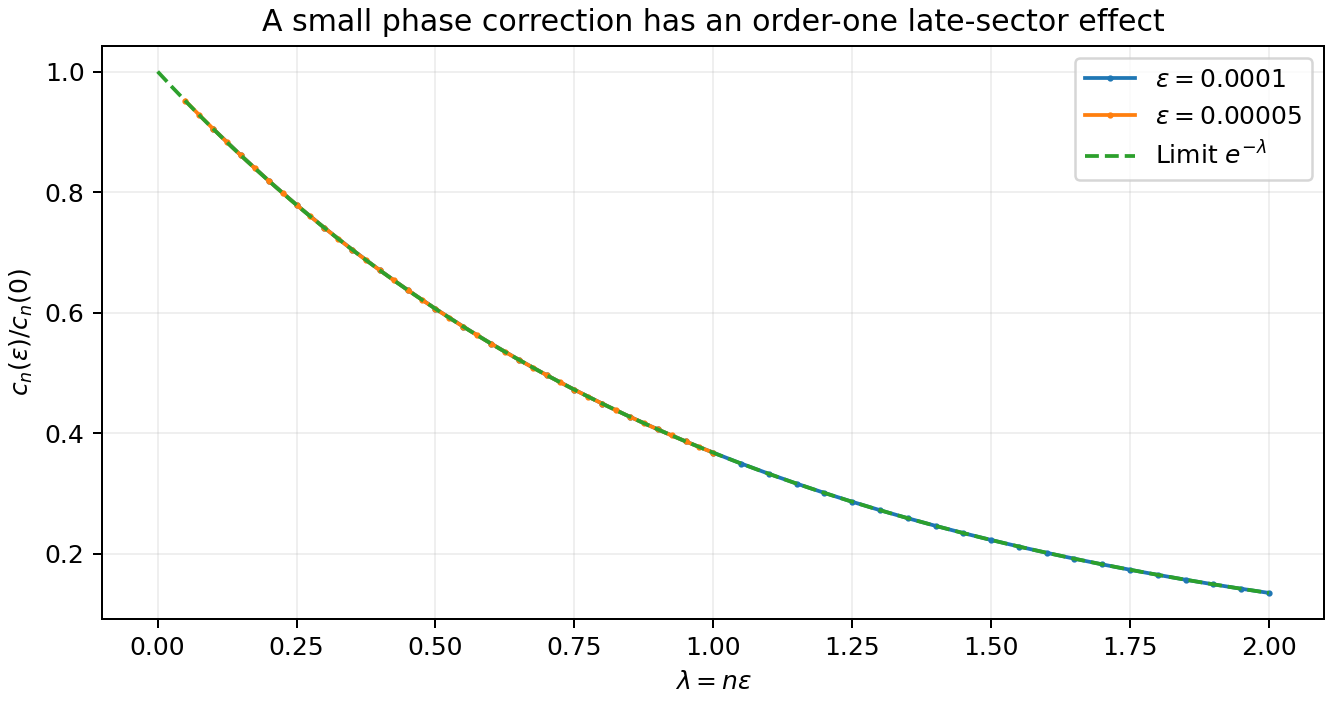
\includegraphics[width=0.91\linewidth]{figures/late_sector_crossover.png}
\caption{The exact finite coefficient formula for $V(s)=\epsilon s^2$ at $\epsilon=10^{-4}$ and $5\times10^{-5}$, compared with the leading crossover profile $\exp(-n\epsilon)$. A small displacement of the convergence radius becomes an order-one change when the sector order is comparable with $\epsilon^{-1}$. This is a numerical illustration of the proved joint limit, not a uniform error estimate for every plotted point.}
\label{fig:crossover}
\end{figure}

\begin{corollary}[Curvature scale for a logarithmic core]
\label{cor:log-crossover}
For the normalized core \eqref{eq:logpsi}, let $a\in\R$, $A>0$ be fixed, let $g\to+\infty$, and let $n\to\infty$ with $n/g^2\to\lambda\in[0,\infty)$. Then
\begin{equation}
 \frac{c_n(g)}{-n^{n-1}/n!}
 \longrightarrow\exp\left(-\frac{a\lambda}{2A}\right).
 \label{eq:log-crossover}
\end{equation}
\end{corollary}
\begin{proof}
The normalized function is jointly holomorphic in $s$ and $h=1/g$ near $h=0$, with removable values there. The uniform lemma applies. From \eqref{eq:log-radius},
$\log(\qcv(g)/\e^{-1})=a/(2Ag^2)+O(g^{-3})$.
Use the uniform leading coefficient formula, noting that $n/g^3\to0$ and $b_1(g)\to\sqrt2$.
\end{proof}

For each fixed sector order $n$, the coefficients tend to the Lambert coefficients as $g\to\infty$. \Cref{cor:log-crossover} explains why this fixed-order convergence cannot be treated as uniform over all sector orders. The natural transition occurs at $n\asymp g^2$, exactly where the small curvature shift is multiplied by a large coefficient index.

\section{Foreign critical values and the failure of a global minimum rule}
\label{sec:foreign}
A tempting but incorrect rule is to find all critical values of the forward function and take the smallest modulus as the radius of every inverse germ. Inversion is sheet-dependent. The next entire example makes the discrepancy arbitrarily large while remaining within the proved exact-radius class.

\begin{theorem}[A much nearer critical value on another sheet]
\label{thm:foreign}
Let
\begin{equation}
 Q_\epsilon(s)=-s\exp(s+\epsilon s^2),
 \qquad 0<\epsilon\leq1/9000.
 \label{eq:quadratic-Q}
\end{equation}
The inverse germ at $q=0$, $s=0$, has radius $\qcv=Q_\epsilon(\scv)$, where
\begin{equation}
 \scv=\frac{-1+\sqrt{1-8\epsilon}}{4\epsilon}
      =-\frac{2}{1+\sqrt{1-8\epsilon}}.
 \label{eq:quadratic-sc}
\end{equation}
The other critical point and its value are
\begin{equation}
 s_{\mathrm f}=\frac{-1-\sqrt{1-8\epsilon}}{4\epsilon},
 \qquad q_{\mathrm f}=-s_{\mathrm f}
                       \exp\bigl((s_{\mathrm f}-1)/2\bigr).
 \label{eq:foreign-critical}
\end{equation}
They satisfy $0<q_{\mathrm f}<\qcv$, and
\begin{equation}
 q_{\mathrm f}\sim\frac1{2\epsilon}\exp\left(-\frac1{4\epsilon}\right),
 \qquad \qcv\longrightarrow\e^{-1}.
 \label{eq:foreign-asymptotic}
\end{equation}
Nevertheless the selected inverse is holomorphic at $q=q_{\mathrm f}$.
\end{theorem}
\begin{proof}
Take $\delta=1/2$. The norm of $V(s)=\epsilon s^2$ on $|s|\leq1.5$ is $2.25\epsilon\leq0.00025$, so \cref{thm:lambert} applies. The critical equation is
$1+s+2\epsilon s^2=0$, giving exactly the two roots displayed. The root near $-1$ is the selected critical point. At either critical root,
$\epsilon s^2=-(1+s)/2$, so $s+\epsilon s^2=(s-1)/2$, proving the value formula.

Both roots are negative. On the interval $(s_{\mathrm f},\scv)$ the quadratic $1+s+2\epsilon s^2$ is negative; hence $Q_\epsilon'(s)>0$. This proves $q_{\mathrm f}<\qcv$. Expanding the far root gives
$s_{\mathrm f}=-1/(2\epsilon)+1+O(\epsilon)$, which yields \eqref{eq:foreign-asymptotic}. Since $q_{\mathrm f}$ lies strictly inside the amplitude disk from the main theorem, the selected inverse is holomorphic there. Its preimage is the unique root in $|s|<|\scv|$, not the far critical point.
\end{proof}

At $\epsilon=10^{-4}$, high-precision evaluation gives
\begin{align*}
 \scv&\simeq-1.00020008004002241344845349486,\\
 \qcv&\simeq0.367916238315796484723861236692,\\
 s_{\mathrm f}&\simeq-4998.99979991995997758655155,\\
 \log_{10}(q_{\mathrm f}/\qcv)&\simeq-1081.60302714816425145.
\end{align*}
The scale of the discrepancy can also be bounded without trusting the displayed decimals. The exact formula gives $4998<-s_{\mathrm f}<5000$, while $\qcv>Q_\epsilon(-1)>\e^{-1}$. Hence
\begin{equation}
 \frac{q_{\mathrm f}}{\qcv}<5000\e^{-2498.5}<10^{-1081}.
 \label{eq:foreign-certified-scale}
\end{equation}
For the last inequality, $\log5000<8.52$ and $\log10<2.303$ suffice, since $8.52+1081(2.303)<2498.5$. The verification script checks these two logarithmic bounds by exact rational lower Taylor sums for the exponential. Thus the greater-than-$10^{1081}$ discrepancy has an elementary certificate; the further digits above remain numerical diagnostics.

\subsection{An exact coefficient formula}
Lagrange inversion for \eqref{eq:quadratic-Q} gives the finite expression
\begin{equation}
 c_n(\epsilon)=\frac{(-1)^n}{n}
 \sum_{k=0}^{\lfloor(n-1)/2\rfloor}
 \frac{(-n\epsilon)^k(-n)^{n-1-2k}}
      {k!(n-1-2k)!}.
 \label{eq:quadratic-cn}
\end{equation}
The first six coefficients are
\begin{align*}
 c_1&=-1,&c_2&=-1,&c_3&=\epsilon-\frac32,\\
 c_4&=4\epsilon-\frac83,&
 c_5&=-\frac52\epsilon^2+\frac{25}2\epsilon-\frac{125}{24},&
 c_6&=-18\epsilon^2+36\epsilon-\frac{54}5.
\end{align*}
For numerical comparison with the Lambert coefficients, division by $c_n(0)$ yields
\begin{equation}
 \frac{c_n(\epsilon)}{c_n(0)}=
 \sum_{k=0}^{\lfloor(n-1)/2\rfloor}
 \frac{(-\epsilon/n)^k}{k!}
 \frac{(n-1)!}{(n-1-2k)!}.
 \label{eq:quadratic-ratio}
\end{equation}
This formula also independently suggests the first crossover: with $n\epsilon\to\lambda$, each fixed summand tends to $(-\lambda)^k/k!$. The proof in \cref{thm:crossover} avoids having to justify this particular exchange of a growing finite sum and a limit.

The same example appears naturally in the transseries problem
$z+\sigma\e^{-z^2}=g$ after the normalization in \cref{sec:actions}. Consequently the foreign-sheet phenomenon is not an artifact of inserting an unrelated entire function.

\subsection{No finite coefficient list determines the exact radius}
\begin{proposition}[A finite-jet obstruction]
\label{prop:finitejet}
For every positive integer $N$, there are two functions satisfying the hypotheses of \cref{thm:lambert} whose selected inverse Taylor series agree through degree $N$ but have different radii of convergence.
\end{proposition}
\begin{proof}
Compare $Q_0(s)=-s\e^s$ with
$Q_u(s)=-s\exp(s+us^N)$ for sufficiently small nonzero real $u$. Their difference is $O(s^{N+1})$, so formal coefficient recursion gives identical inverse coefficients through degree $N$. Their inverse derivatives at zero are both $-1$, so there is no degeneracy. On the other hand, \eqref{eq:qc-smallparameter} gives
\[
 \qcv(u)=\e^{-1}\bigl(1+(-1)^Nu+O(u^2)\bigr).
\]
For sufficiently small real $u\neq0$, this differs from $\e^{-1}$. The norm condition holds after making $u$ small enough, so these critical values are the exact radii.
\end{proof}

Finite symbolic jets are valuable for computing coefficients, but they cannot, by themselves, certify a global analytic radius. The extra information in the main theorem is a norm bound on a disk reaching the fold, not an unusually long list of low-order coefficients.

\section{Sectorial gluing, Stokes transitions, and inversion}
\label{sec:stokes}
The preceding theorems describe selected local analytic branches. They fit into a sectorial theory when the charts are glued with their domains and summation data intact. This section gives precise compatibility identities; it does not claim that every formal complex transseries is summable.

\subsection{Coordinate transitions have an order}
Let $F_-$ and $F_+$ be locally biholomorphic sectorial realizations on compatible source charts, with selected inverses $G_-$ and $G_+$. On a common target chart define
\begin{equation}
 J=F_+\circ G_-.
 \label{eq:J}
\end{equation}
Then, wherever the compositions stay on the selected charts,
\begin{equation}
 F_+=J\circ F_-\qquad\Longrightarrow\qquad
 G_+=G_-\circ J^{-1}.
 \label{eq:inverse-gluing}
\end{equation}
This is an identity of analytic coordinate maps. It follows simply by composing with the specified inverses, but it prevents an important error: inversion is not performed by subtracting the forward jump at the same target argument.

For a compatible family, put $J_{\alpha\beta}=F_\alpha\circ G_\beta$. Then
\begin{equation}
 J_{\alpha\beta}\circ J_{\beta\gamma}=J_{\alpha\gamma}
 \label{eq:cocycle}
\end{equation}
on triple overlaps, and the inverse charts obey the reversed composition rule in \eqref{eq:inverse-gluing}. These identities concern genuine coordinate transitions. A Stokes automorphism on a formal algebra is related to them only after its realization and its action on the chosen functions have been specified.

\subsection{The nonlinear inverse jump}
For a small perturbation $F_\varepsilon(z)=F(z)+\varepsilon H(z)$, fix $w$, set $g=G(w)$, and assume a common noncritical inverse neighborhood. Taylor expansion gives
\begin{equation}
 \begin{split}
 G_\varepsilon(w)=g
 &-\varepsilon\frac{H(g)}{F'(g)}\\
 &+\varepsilon^2\left(
       \frac{H(g)H'(g)}{F'(g)^2}
       -\frac{F''(g)H(g)^2}{2F'(g)^3}\right)
 +O(\varepsilon^3).
 \end{split}
 \label{eq:inverse-jump}
\end{equation}
To verify the formula, substitute $g+\varepsilon u+\varepsilon^2v$ into $F_\varepsilon(z)=w$. The first two equations are
$F'u+H=0$ and $F'v+F''u^2/2+H'u=0$. This familiar formula already shows why a finite Stokes jump is not obtained just by negating a constant: transport, differentiation, and curvature all appear. Near a fold, its denominators signal that the noncritical chart is no longer appropriate.

The repository's exact-core transport results give higher-order versions of this mechanism \cite{repo-stokes}. Equation \eqref{eq:inverse-gluing} explains their coordinate meaning; it is not presented as a new resurgence closure theorem.

\subsection{Transport of the fold between normalized charts}
Suppose two normalized local realizations are represented on the same $s$-disk by $V_-$ and $V_+$, both satisfying the small-norm condition. Let $\Delta V=V_+-V_-$ and interpolate $V_u=V_-+u\Delta V$, $0\leq u\leq1$. The norm bound is convex, so the selected critical point exists along the path. Integrating \eqref{eq:qc-envelope} gives the exact formula
\begin{equation}
 \log\frac{\qcv(1)}{\qcv(0)}
       =\int_0^1\Delta V(\scv(u))\,du,
 \label{eq:fold-jump}
\end{equation}
where the logarithm is continued along the path. In particular, a small perturbation has the first variation
\begin{equation}
 \delta\log\qcv=\delta V(\scv)
            +O(\norm{\delta V}^{\,2}),
 \label{eq:fold-linear}
\end{equation}
with the norm taken on the fixed larger disk and constants depending on the fixed disk margin. Cauchy's estimates and \eqref{eq:sc-variation} justify the quadratic remainder. This is a selected-fold sensitivity formula. It becomes a Stokes transport formula only when $V_\pm$ actually arise from specified lateral realizations in a common normalization. If the normalizing scales differ, their changes must also be included through \eqref{eq:radius-sigma}.

\subsection{What established resurgence closure contributes}
In a standard setting one specifies a closed discrete additive set of Borel singularities containing zero, an algebra of resurgent germs relative to that set, and appropriate tangent-to-identity behavior at infinity. Sauzin proves closure under the relevant nonlinear operations and functional inversion \cite{sauzin}. Directional summation then identifies the admitted formal expressions with their selected analytic realizations under the theorem's hypotheses.

Those results cannot be replaced by the statement that every complex action series is resurgent. A countable action set may fail local finiteness or accumulate; a direction may cease to be admissible; an oscillatory substitution may leave the formal algebra. The critical-circle theorem requires an actual holomorphic normalized map. It can be applied after a resurgent or multisummable construction supplies that map, but does not manufacture the missing summation structure.

Globally, further obstructions include multiple preimages, accessible critical values, finite asymptotic values of a continued forward map, and boundaries of its domain. The example in \cref{sec:foreign} shows why the word ``accessible'' must refer to the selected sheet. Our theorem settles a local but nontrivial region of this global problem.

\section{Computation, reproducibility, and the proof boundary}
\label{sec:computation}
\subsection{A practical sequence of checks}
For an inverse problem of the form \eqref{eq:generalaction}, a reliable calculation begins with a core value $g$, a source disk, and explicit logarithm branches. Compute the effective slope \eqref{eq:effective-slope}; if it vanishes, choose another leading model rather than forcing this one. Construct $\psi$, $B$, and $V$ exactly. An estimate such as \eqref{eq:V-certificate} establishes whether the Lambert-stable theorem applies. Then solve $H=0$ near $-1$, compute the selected critical value, and generate the Puiseux coefficients from \eqref{eq:bk}.

Low-order amplitude coefficients can be computed by Lagrange inversion or coefficient recursion. Large orders are better described by \eqref{eq:cn-all}, with a separately controlled error. An interior evaluation uses \eqref{eq:rough-tail} or a refined bound; near the boundary one uses the square-root chart and \cref{thm:tail}. A residual certificate such as \cref{prop:certificate} can independently validate a numerical approximate root away from the fold. None of these steps should be replaced by selecting the globally smallest critical value.

\subsection{Executed exact checks}
The included \path{verify.py} uses exact symbolic algebra to verify the quadratic example's compositional residual through amplitude degree nine, the general formulas for $b_1,b_2,b_3$ through the corresponding fourth-order local identity, the small-parameter critical-value formula through second order, the normalized logarithmic unit expansion through $g^{-3}$, and the rational exponential inequalities used in \eqref{eq:foreign-certified-scale}. These tests were executed successfully. They are finite checks of displayed formulas, not substitutes for the all-order proofs.

The high-precision calculations use 110 decimal digits. They test the late-sector approximation, the boundary tail, the first crossover, a genuinely complex perturbation, and the foreign critical value. The code records actual outputs in \path{results/verification.json}. Floating-point evaluation and the stopping rule in the finite-sum routine are not directed-rounding interval arithmetic. The analytic theorems, rather than numerical sampling, carry the proof of the radius.

\begin{table}[htbp]
\centering\small
\begin{tabular}{r rr}
\toprule
Sector order $n$ & $c_n\qcv^n n^{3/2}$ & Relative error, two-term formula\\
\midrule
25   & $-0.397730918613220$ & $5.77\times10^{-6}$\\
100  & $-0.398728814691040$ & $3.52\times10^{-7}$\\
400  & $-0.398978696035148$ & $2.19\times10^{-8}$\\
1600 & $-0.399041191092424$ & $1.36\times10^{-9}$\\
\bottomrule
\end{tabular}
\caption{Executed diagnostics for $V(s)=10^{-4}s^2$. The two-term approximation is \eqref{eq:cn-two}; its relative error is expected to be $O(n^{-2})$. The decimals are not interval enclosures.}
\label{tab:late}
\end{table}

For the same example, $b_1\simeq1.4146380457772240673$ and $d_1\simeq-0.0835335235041493284$. The boundary-tail calculation gives
\begin{center}
\small
\begin{tabular}{r r}
\toprule
$N$ & $\sqrt N\bigl(s(\qcv)-S_N(\qcv)\bigr)$\\
\midrule
125 & $-0.796354305922977$\\
500 & $-0.797680809520248$\\
2000 & $-0.798013189501830$\\
Limit from \cref{thm:tail} & $-0.798124049917864$\\
\bottomrule
\end{tabular}
\end{center}
The first-crossover diagnostic at $\epsilon=1/n$ is also recorded. Some of its smaller $n$ values lie outside our conservative sufficient norm bound; those points are numerical comparisons only. For all sufficiently large $n$ the theorem applies, and the proved limit is $\e^{-1}$.

\subsection{Files and reproducible builds}
The accompanying archive contains this \LaTeX{} source, the compiled PDF, the verification program and its recorded JSON output, two generated figures, a source-provenance note, a claim ledger, and build instructions. The article uses ordinary \texttt{pdflatex} with the packages listed in its preamble. The scripts require no network access after their dependencies are installed. The build script writes fresh verification data and generated figures to a separate build directory so the recorded evidence is not silently overwritten.

There is no Lean code in this package and no claim of machine-checked mathematical proofs. A future formalization would need, in addition to coefficient algebra, complex-analytic zero counting, parameterized inverse charts, and the quantitative angular minimum argument. The repository's existing formal coefficient infrastructure may support the algebraic part, but that is not the whole proof.

\section{Further research questions and topics}
\label{sec:questions}
The exact-radius theorem resolves the identified large-core question, but also exposes several concrete next steps. The following problems are proposals from this report; they are not all asserted to be previously published open problems.

\paragraph{1. Determine the sharp Lambert-stability region.}
The constant $\delta^2/1000$ is deliberately small. For a given disk margin, determine the largest norm neighborhood in which a critical circle or another canonical contour proves a unique dominant fold. In the quadratic example, determine exactly how far the selected-radius conclusion persists beyond the sufficient range $0<\epsilon\leq1/9000$, including complex $\epsilon$. The critical-point collision at $\epsilon=1/8$ is a natural landmark, but does not by itself classify every complex-parameter obstruction.

\paragraph{2. Replace circles by adaptable source contours.}
The proof succeeds because a circle through the critical point has a unique minimum of $|Q|$. Develop a contour criterion stable under larger perturbations, with a verified construction from the forward map. Such a criterion could apply when the critical point is still dominant but the circular angular convexity argument fails. A useful target is an effective lower bound for the amplitude domain that becomes exact at a certified accessible critical point.

\paragraph{3. Study several exponential amplitudes simultaneously.}
For $F(z)+\sum_j\sigma_j a_j(z)\e^{-\Phi_j(z)}=w$, the discriminant is a hypersurface in amplitude space. Determine the domain of absolute convergence of the selected multivariate inverse and which discriminant strata control mixed coefficient directions. The analogue of the present positivity-free, sheet-selective argument should distinguish an accessible discriminant from unrelated sheets. Resonant actions must be grouped without changing the amplitude geometry.

\paragraph{4. Extend beyond locally finite action sets.}
Establish nonlinear inversion theorems for specified countable action spaces with accumulation, stating exactly which weighted analytic norms, filtered Borel continuation spaces, and substitution operations are preserved. The target is not merely analytic convergence of a countable sum, but a clearly defined resurgent or generalized summability statement. The existing distinction between action-budget finiteness and analytic weighted completion should remain visible.

\paragraph{5. Develop resurgence of the moving critical geometry.}
When $V_g$ has a divergent but summable coefficient expansion, study the expansions of $s_{\mathrm c}(g)$, $q_{\mathrm c}(g)$, and $b_k(g)$ as resurgent objects. Determine which established implicit-function results apply after the exact core has been extracted. Combine those closure results with \eqref{eq:fold-jump} to compute genuine lateral changes of the fold location, rather than only its formal perturbation coefficients.

\paragraph{6. Classify accessible and foreign inverse singularities.}
Construct an algorithm or a set of verifiable continuation criteria that associates critical and asymptotic values with particular inverse germs. The quadratic example proves that sorting all critical values by modulus is insufficient. A next target is a finite description for polynomial times exponential maps, followed by maps built from logarithmic cores. The output should include monodromy information and domain restrictions, not just a list of critical values.

\paragraph{7. Treat higher-order critical points and competing folds.}
When $H'(s_{\mathrm c})=0$, a square root is no longer the correct local coordinate. Prove an exact-dominance theorem for a selected $m$th-order branch point under suitable global contour conditions, and derive the corresponding $n^{-1-1/m}$ coefficient law. For nearly coalescing critical points, identify the uniform local algebraic model and the coefficient scaling regime; the model must be derived rather than assumed from an analogy with saddle-point integrals.

\paragraph{8. Couple late-sector order with divergent inner expansions.}
The current joint limit has a convergent analytic parameter $1/g$ for the pure logarithmic core. Extend it to Gevrey or multisummable coefficient algebras and quantify how optimal truncation in the core variable interacts with the late amplitude index. A useful theorem would control both errors uniformly through $n\asymp g^2$ and explain when an exponentially small core ambiguity is amplified by high sector order.

\paragraph{9. Build a compatible atlas for oscillatory and nested actions.}
Specify sectors, logarithmic sheets, action dominance, and allowable substitutions for a genuinely complex transseries atlas. Determine how the exact-core construction changes as an action rotates from decaying to oscillatory. The goal is a concrete gluing theorem with stated hypotheses, not a total ordering of all complex transmonomials on the entire plane.

\paragraph{10. Minimize the analytic information needed for certification.}
\Cref{prop:finitejet} shows that no finite coefficient list determines an exact radius. Determine useful combinations of finite jets, norm bounds, and a small amount of contour information that do. This could lead to a practical certificate format with explicit rational inequalities and an independently checkable root-selection witness.

\paragraph{11. Formalize the analytic geometry.}
A focused Lean development could first formalize the derivative-disk certificate, the critical-circle angular inequality, and the Rouch\'e root count. The next stage is parameterized continuation and the selection of the inward Puiseux branch. Keeping the formal statement sheet-specific would prevent the foreign-critical-value error by construction.

\paragraph{12. Investigate exact finite-core radii in the repository models.}
The present result applies to sufficiently large core parameters. For the Euler--logarithm and inverse-harmonic models already in the repository, determine the remaining finite parameter intervals, including where other singularities become accessible. This requires additional global analytic information; it cannot be inferred solely by extending an asymptotic fold formula to smaller parameters.

\section{Conclusion}
A theory of reversion for complex transseries must preserve three distinctions: formal versus analytic inversion, exponential-amplitude convergence versus coefficient asymptotics, and selected-sheet singularities versus all critical values of a forward map. The critical-circle theorem makes these distinctions productive rather than merely cautionary. A small, explicitly bounded analytic perturbation of the Lambert model has a unique dominant fold on the selected inverse sheet, even for complex perturbations without coefficient positivity. This supplies the exact radius missing from the inspected large-core analysis.

The consequence is more than a radius formula. It gives a full late-sector expansion, a boundary tail profile, a curvature-dependent crossover, and a normalization accommodating nonlinear actions and prefactors. The foreign-sheet example shows why the selection proof is essential. Extending these results to larger perturbations, several actions, and global sectorial atlases remains a well-defined research program rather than an unsupported claim of universal closure.

\appendix
\section{Notation and logical dependencies}
\label{app:notation}
\begin{center}\small
\begin{tabular}{>{\raggedright\arraybackslash}p{0.19\linewidth}p{0.73\linewidth}}
\toprule
Symbol & Meaning\\
\midrule
$g$ & Fixed core preimage; often tends to infinity in a later asymptotic limit.\\
$z$ & Original source variable of the inversion problem.\\
$s$ & Normalized inverse displacement; also $s(q)$ for its selected branch.\\
$q,\sigma$ & Normalized and original exponential amplitudes.\\
$\alpha$ & Effective local action slope, including the prefactor correction.\\
$\psi,B,V$ & Normalized core, effective action increment, and logarithmic perturbation.\\
$Q$ & Forward normalized amplitude map $-s\exp(s+V(s))$.\\
$H$ & Critical equation $1+s+sV'(s)$.\\
$\scv,\qcv$ & Selected critical point near $-1$ and its critical value.\\
$c_n,b_k$ & Taylor amplitude coefficients and local Puiseux coefficients.\\
$u$ & An analytic perturbation parameter, not an action index.\\
\bottomrule
\end{tabular}
\end{center}

The formal theorem in \cref{sec:formal} and the analytic certificate in \cref{sec:certificates} are independent preliminary frameworks. The exact-radius theorem depends only on the holomorphy and norm condition in \eqref{eq:smallV}. Late coefficients and tails additionally use classical singularity transfer. Nonlinear-action and repository applications depend on proving the normalization meets the same norm condition. The joint limits additionally use uniform analytic parameter dependence. Stokes interpretations require separate realization and summation hypotheses. Numerical tests are downstream checks and do not appear as assumptions in any proof.

\section{A compact claim ledger}
\label{app:ledger}
\begin{center}\small
\begin{tabular}{>{\raggedright\arraybackslash}p{0.35\linewidth}p{0.57\linewidth}}
\toprule
Claim & Status and boundary\\
\midrule
Critical-circle and exact-radius theorem & Proved here for the explicit disk-norm class, including complex perturbations.\\
Large-core repository radius equality & Proved consequence under complex-uniform hypotheses; no assertion for every smaller finite core value.\\
Late coefficients and boundary profile & Proved from the geometric theorem and classical transfer; not a new general transfer principle.\\
Nonlinear-action normalization & Exact local algebra with a sufficient analytic certificate; excludes zero effective slope.\\
Critical-value sensitivity and crossovers & Proved identities and uniform limits within analytic families.\\
Foreign-sheet example & Explicit exact model; inequality and radius proved, decimal size numerically evaluated.\\
Formal reversion and resurgence closure & Formal sufficient framework proved; established resurgence theorems credited, not generalized without hypotheses.\\
Symbolic and numerical verification & Executed finite checks; no interval enclosure or Lean verification claimed.\\
Literature novelty & Proposed contribution and repository gap resolution; independent priority not established.\\
\bottomrule
\end{tabular}
\end{center}

\clearpage
\phantomsection
\addcontentsline{toc}{section}{References}
\begin{thebibliography}{9}
\bibitem{sauzin}
David Sauzin, \emph{Nonlinear analysis with resurgent functions},
Annales scientifiques de l'\'Ecole normale sup\'erieure (4) \textbf{48} (2015), no.~3, 667--702.
DOI: \href{https://doi.org/10.24033/asens.2255}{10.24033/asens.2255}.
Author's preprint: \url{https://arxiv.org/html/1212.4477v4}.

\bibitem{dlmf}
NIST Digital Library of Mathematical Functions, \S4.13, \emph{Lambert $W$-function}.
\url{https://dlmf.nist.gov/4.13}. Accessed 4 October 2026.

\bibitem{fs}
Philippe Flajolet and Robert Sedgewick, \emph{Analytic Combinatorics},
Cambridge University Press, 2009, especially Chapter VI, singularity analysis.
Author-maintained companion site: \url{https://ac.cs.princeton.edu/home/}.

\bibitem{vdh-complex}
Joris van der Hoeven, \emph{Complex transseries solutions to algebraic differential equations}, author-hosted manuscript.
\url{https://www.texmacs.org/joris/osc/osc.html}. Accessed 4 October 2026.

\bibitem{repo-stokes}
\repo{} repository, \emph{Nonlinear Stokes Transport under Logarithmic Inversion},
report dated 29 September 2026, with repository editorial amendments.
Files \path{README.md} and \path{article.tex}, especially the theorem labelled \texttt{thm:radius}, under
\path{Analysis/Transseries/docs/series-and-transseries/Nonlinear_Stokes_Transport_Logarithmic_Inversion/}.
Repository: \url{https://github.com/VladimirReshetnikov/ProveIt}.
Comparison revision \texttt{6cb1d86f19ebf9f54c8d985b141b84233b6eab66}.

\bibitem{repo-moments}
\repo{} repository, \path{Moment_Determinacy_Nonlinear_Transseries} package,
files \path{CLAIM_LEDGER.md} and \path{moment_determinacy_transseries.tex} in
\path{Analysis/Transseries/docs/series-and-transseries/Moment_Determinacy_Nonlinear_Transseries/}, same comparison revision as \cite{repo-stokes}.

\end{thebibliography}
\end{document}
